\documentclass{article}\usepackage[T1]{fontenc}

\usepackage[utf8]{inputenc}
\usepackage{graphicx}

\usepackage{lmodern}
\begin{document}
\title{APMA 4301: Problem Set 4b}
\author{Brian Dawes}
\maketitle

The number of ksp iterations for each solver and solver time per degree of freedom ($N^2$) for $N=8,16,32,64$ can be found in the below table. The convergence for $N=64$ can be seen in the below graph.

From the graph, we can see that the LU preconditioned Richardson solves the problem exactly in one step. The two GAMG solvers converge the quickest out of the iterative solvers with CG slightly faster than Richardson. The next quickest are the ILU preconditioned methods, with CG slightly faster than GMRES. CG with no preconditioner is converging to the solution slowly, while unpreconditioned GMRES and SOR preconditioned Richardson both do not appear to be converging (or at least are converging very very slowly).

From the table, we see that the LU solvers converge the quickest. Out of the iterative methods, the two GAMG solvers converge the quickest. Since this problem is not very large, the LU sparse direct solvers are the optimal way to solve the problem, with umfpack being the faster of the two. However, as the size of the problem increases, the GAMG preconditioned solvers begin to perform similarly to the LU solvers, indicating that these may be the optimal choice for larger problems.
 
\begin{tabular}{crrlll}
\hline
Solver&nCells&nIts&$||r||_2$&$||e||_2$&KSP time/DoF (s)\\
\hline
lu-richardson-umfpack&8&1&5.884e-15&1.067729e-03&1.037e-05\\
lu-richardson-umfpack&16&1&1.475e-14&2.729133e-04&2.910e-06\\
lu-richardson-umfpack&32&1&3.710e-14&6.885276e-05&9.990e-07\\
lu-richardson-umfpack&64&1&8.125e-14&1.728282e-05&2.458e-07\\ \hline
lu-richardson-mumps&8&1&9.491e-15&1.067729e-03&3.358e-05\\
lu-richardson-mumps&16&1&2.096e-14&2.729133e-04&1.492e-05\\
lu-richardson-mumps&32&1&3.694e-14&6.885276e-05&3.105e-05\\
lu-richardson-mumps&64&1&8.026e-14&1.728282e-05&2.900e-05\\ \hline
sor-richardson-none&8&113&4.999e-09&1.067731e-03&1.468e-03\\
sor-richardson-none&16&200&1.303e-04&3.854372e-04&6.916e-04\\
sor-richardson-none&32&200&7.146e-02&1.874269e-01&1.478e-04\\
sor-richardson-none&64&200&2.162e-01&1.117586e+00&1.055e-04\\ \hline
none-cg-none&8&34&9.482e-09&1.067729e-03&3.078e-04\\
none-cg-none&16&70&1.331e-08&2.729133e-04&2.669e-04\\
none-cg-none&32&138&2.076e-08&6.885277e-05&7.127e-05\\
none-cg-none&64&200&3.478e-05&1.869412e-05&1.344e-04\\ \hline
none-gmres-none&8&35&6.620e-09&1.067729e-03&1.561e-04\\
none-gmres-none&16&108&1.449e-08&2.729212e-04&4.288e-04\\
none-gmres-none&32&200&2.417e-06&7.169367e-05&3.126e-04\\
none-gmres-none&64&200&1.321e-02&6.188559e-02&1.254e-04\\ \hline
ilu-cg-none&8&12&6.463e-09&1.067729e-03&1.684e-04\\
ilu-cg-none&16&20&9.301e-09&2.729134e-04&5.261e-05\\
ilu-cg-none&32&35&2.147e-08&6.885273e-05&4.023e-05\\
ilu-cg-none&64&69&2.410e-08&1.728281e-05&2.271e-05\\ \hline
ilu-gmres-none&8&12&6.800e-09&1.067729e-03&9.381e-05\\
ilu-gmres-none&16&20&1.120e-08&2.729134e-04&3.668e-05\\
ilu-gmres-none&32&38&1.063e-08&6.885300e-05&3.229e-05\\
ilu-gmres-none&64&98&2.011e-08&1.728412e-05&7.492e-05\\ \hline
gamg-cg-none&8&8&1.452e-08&1.067729e-03&1.287e-04\\
gamg-cg-none&16&9&8.700e-09&2.729134e-04&3.658e-05\\
gamg-cg-none&32&9&5.198e-08&6.885250e-05&7.754e-06\\
gamg-cg-none&64&10&1.188e-08&1.728281e-05&8.274e-06\\ \hline
gamg-richardson-none&8&14&1.836e-08&1.067730e-03&1.029e-04\\
gamg-richardson-none&16&18&5.672e-09&2.729139e-04&3.380e-05\\
gamg-richardson-none&32&18&1.536e-08&6.885382e-05&3.172e-05\\
gamg-richardson-none&64&18&1.377e-08&1.728375e-05&6.999e-06\\
\hline\end{tabular}

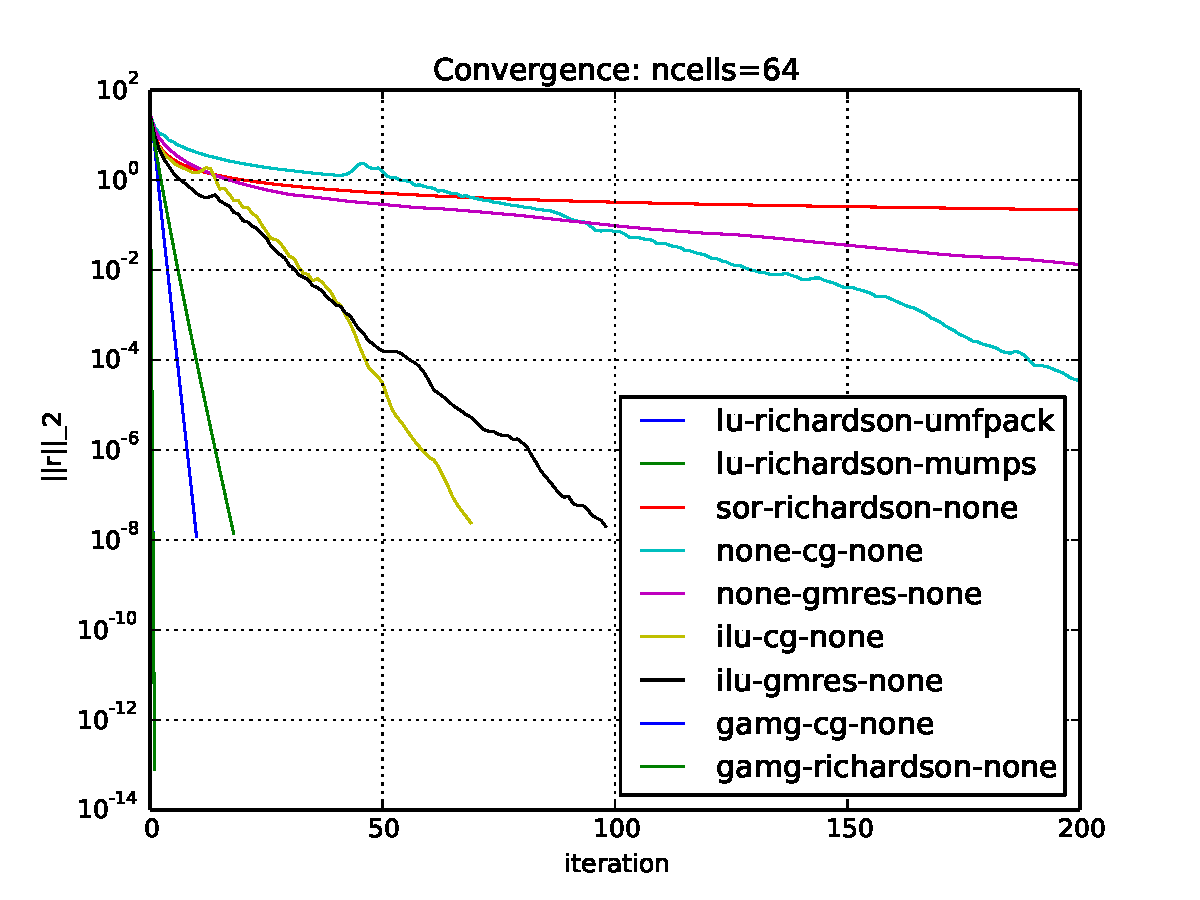
\includegraphics[width=\linewidth]{convergence.pdf}
\end{document}